\documentclass{beamer}
\usepackage{ctex, hyperref}
\usepackage[T1]{fontenc}
\newcommand{\team}{Team \#\ {2024050727407}, Problem B}
\usepackage{latexsym,amsmath,xcolor,multicol,booktabs,calligra}
\usepackage{graphicx,pstricks,listings,stackengine, ragged2e}
\usepackage{tikz}
\usetikzlibrary{positioning, arrows.meta}
\newcommand{\upcite}[1]{\textsuperscript{\textsuperscript{ \cite{#1}}}}
\author[答辩人:陆子凯、狄诗琪]{答辩人:陆子凯、狄诗琪 \\ 指导教师:赵英姿} % [短版本]用于footline,{长版本}用于titlepage
\title{生物质和煤共热解技术中特征选择和优化研究}
\subtitle{\raisebox{-0.28\height}{
\includegraphics[height=1.6em]{pic/logo.png}}2024年第九届"数维杯"大学生数学建模挑战赛论文答辩}
\institute{\team}
\date{2024年9月23日}
\usepackage{JOU}

% defs
\def\cmd#1{\texttt{\color{red}\footnotesize $\backslash$#1}}
\def\env#1{\texttt{\color{blue}\footnotesize #1}}
\definecolor{deepblue}{rgb}{0,0,0.5}
\definecolor{deepred}{rgb}{0.6,0,0}
\definecolor{deepgreen}{rgb}{0,0.5,0}
\definecolor{halfgray}{gray}{0.55}

\lstset{
    basicstyle=\ttfamily\small,
    keywordstyle=\bfseries\color{deepblue},
    emphstyle=\ttfamily\color{deepred},
    stringstyle=\color{deepgreen},
    numbers=left,
    numberstyle=\small\color{halfgray},
    rulesepcolor=\color{red!20!green!20!blue!20},
    frame=shadowbox,
}

\begin{document}

\kaishu
\begin{frame}
    \titlepage
    \begin{figure}[htpb]
        \centering
        \vspace{-5mm}
        
\includegraphics[width=0.22\linewidth]{pic/JOU_logo.jpg}
    \end{figure}
\end{frame}

\begin{frame}
    \tableofcontents[sectionstyle=show,subsectionstyle=show/shaded/hide,subsubsectionstyle=show/shaded/hide]
\end{frame}

% 引言
\section{引言}
\subsection{研究背景}
\begin{frame}{研究背景}
    \justifying
    \begin{columns}
        \column{0.6\textwidth}
        \begin{itemize}
            \item 全球能源需求的增长与环境问题的日益严重,开发清洁、高效的可再生能源成为关键。
            \item 生物质是一种丰富的可再生资源,与煤共热解可利用两者的协同效应,提高产物质量和能源转化效率。
        \end{itemize}
        \column{0.4\textwidth}
        \begin{figure}[htbp]
            \centering
            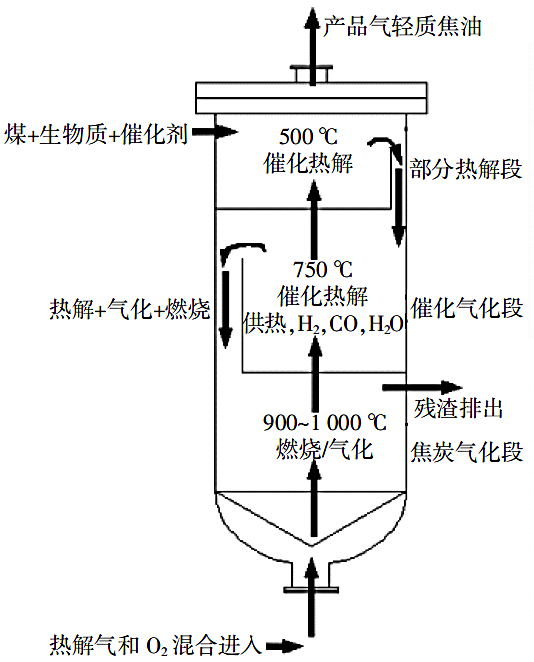
\includegraphics[width=\linewidth]{pic/工艺示意图.png}
            \caption{生物质与煤共热解工艺示意图\upcite{ref13}}
        \end{figure}
    \end{columns}
\end{frame}

\subsection{研究目的与意义}
\begin{frame}{研究目的与意义}
    \justifying
    \begin{columns}
        \column{0.5\textwidth}
        \begin{block}{研究目的}
            \begin{itemize}
                \item 探究生物质与煤共热解过程中影响产物组成和产率的关键因素。
                \item 建立数学模型,优化共热解工艺参数,提高产物质量和能源转化效率。
            \end{itemize}
        \end{block}
        \column{0.5\textwidth}
        \begin{block}{研究意义}
            \begin{itemize}
                \item 为共热解技术的工业应用提供理论指导,推动技术进步。
                \item 促进可再生能源的开发利用,优化能源结构,减少环境污染。
            \end{itemize}
        \end{block}
    \end{columns}
\end{frame}

% 问题重述
\section{问题重述与分析}
\begin{frame}{问题重述}
    \justifying
    \begin{enumerate}[<+->]
        \item \textbf{问题一}:分析正己烷不溶物(INS)对各热解产物产率的影响。
        \item \textbf{问题二}:研究 INS 及其与混合比例的交互效应对产物组成的影响。
        \item \textbf{问题三}:确定最佳混合比例,提升产物利用率与能源转化效率。
        \item \textbf{问题四}:分析产物收率的实验值与理论值差异及其分布规律。
        \item \textbf{问题五}:建立热解产物产率的预测模型,提高工艺控制精度。
    \end{enumerate}
\end{frame}
\begin{frame}{问题分析}
    \justifying
    \begin{figure}[htbp]
        \centering
        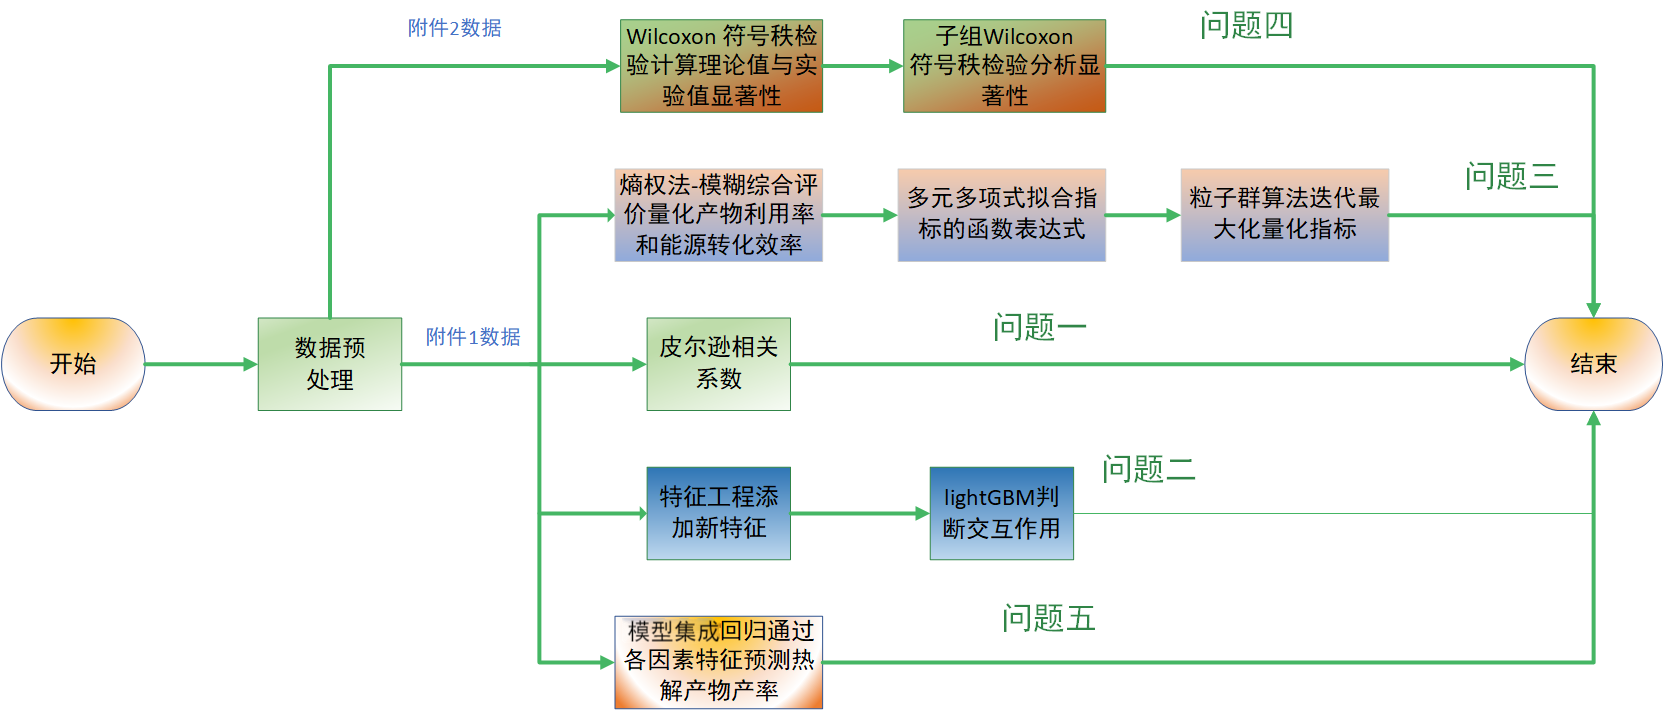
\includegraphics[width=0.94\linewidth]{pic/问题分析.png} % 调整图片大小以适应幻灯片
        \caption{问题分析流程图}
        \label{fig:problem-analysis}
    \end{figure}
\end{frame}


% 数据预处理与探索性分析
\section{数据预处理与探索性分析}

\subsection{数据预处理}
\begin{frame}{数据预处理}
    \justifying
    \alert{附件数据缺失}是影响分析质量的重要因素,而直接忽视缺失值可能导致结果偏差,甚至使模型失效。
    \vspace{0.25cm}
    针对附件一中缺失的正己烷不溶物(INS)数据,我们通过观察变量间的统计关系,采用\alert{线性插值法}进行处理。正己烷不溶物与焦油比率数据波动较小(如表 \ref{tab:chemical_ratios}),显示出潜在的线性关系,因此线性插值法能够较好地补足缺失值,保持数据连续性。
    \vspace{0.25cm}
    对于附件二中的实验数据缺失,考虑到混合比例下数据可能呈现更复杂的趋势,我们选择了\alert{Lagrange插值法}。该方法通过构建插值多项式,能够更好地拟合非线性关系,提高了缺失数据的估计精度。
    \vspace{0.25cm}    
    最后,我们对数据进行了重构转换,将混合比例从生物质/煤的比例形式转换为\alert{生物质/(生物质+煤)}的小数格式,以提高数据处理的一致性与\alert{数值计算}的便捷性。
\end{frame}

\begin{frame}{缺失值处理方法}
    \justifying
    在数据预处理中,INS 数据缺失的处理尤为关键。表 \ref{tab:chemical_ratios} 展示了正己烷不溶物与其他变量间的化学比率统计数据。根据这些比率的一致性,我们选择了线性插值来填补缺失数据。
    
    \vspace{0.1cm}
    \begin{table}[htbp]
    \centering
    \caption{化学比率的统计数据}
    \begin{tabular}{cccc}
    \hline
    \textbf{化学比率} & \textbf{平均值} & \textbf{中位数} & \textbf{标准差} \\
    \hline
    正己烷不溶物/焦油比率 & 0.283 & 0.280 & 0.106 \\
    正己烷可溶物/焦油产率比率 & 0.805 & 0.758 & 0.510 \\
    正己烷不溶物/水比率 & 0.313 & 0.284 & 0.186 \\
    焦渣产率/水产率比率 & 5.909 & 5.869 & 2.300 \\
    \hline
    \end{tabular}
    \label{tab:chemical_ratios}
    \end{table}
    
    针对实验数据的缺失,通过应用Lagrange插值对缺失实验数据进行估计,以确保插值结果不会偏离数据的总体趋势。
\end{frame}

\begin{frame}{数据结构}
    \justifying
    下图\ref{fig:dataset_structure}展示了数据预处理后中 135 个样本的部分变量和对应的数值。
    \vspace{0.3cm}
    \begin{figure}[htbp]
        \centering
        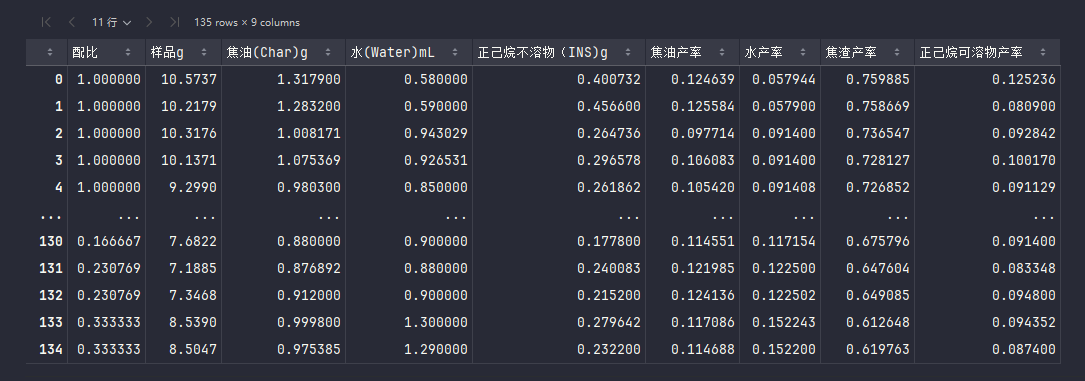
\includegraphics[width=0.9\linewidth]{pic/数据结构.png} % 使用实际文件路径替换
        \caption{数据结构}
        \label{fig:dataset_structure}
    \end{figure}
\end{frame}

\subsection{探索性数据分析}
\begin{frame}{探索性数据分析}
    \justifying
    数据预处理完成后,探索性数据分析(EDA)是进一步理解数据特征及其潜在规律的关键步骤。通过对描述性统计和相关性分析的深入探索,我们能够识别变量之间的关联性,并为后续模型构建提供可靠依据。
    
    表 \ref{tab:descirption} 提供了部分变量的主要统计特征。其中,焦油产率的均值为 15.2,标准差为 2.5\%。通过皮尔逊相关性分析,我们发现 INS 含量与焦油产率的相关性较强(相关系数为 0.65),提示 INS 含量可能是影响焦油产率的重要因素。

    \begin{table}[htbp]
    \centering
    \caption{描述性统计数据}
    \label{tab:descirption}
    \small
    \begin{tabular}{@{}cccccccc@{}}
    \hline
    \textbf{变量名} & \textbf{样本量} & \textbf{最大值} & \textbf{最小值} & \textbf{平均值} & \textbf{标准差} \\
    \hline
    配比 & 135 & 1.00 & 0.048 & 0.295 & 0.301 \\
    焦油 g & 135 & 2.139 & 0.361 & 1.038 & 0.316 \\
    水 mL & 135 & 1.91 & 0.58 & 1.037 & 0.295 \\
    INS g & 135 & 0.935 & 0.025 & 0.304 & 0.158 \\
    \hline
    \end{tabular}
    \end{table}
\end{frame}

\begin{frame}{数据可视化分析}
    \justifying
    通过可视化分析,数据的分布和变量间关系得到了更为直观的展示。图 \ref{fig:boxplot} 显示了焦油、水、INS 等关键变量的箱线图,从中可以观察到变量的集中趋势及其潜在的异常点,各指标均不能通过正态性检验,所以在相关性分析前进行了Z-score 标准化使数据具备标准正态分布的特征(均值为0,标准差为1)。

    \vspace{1cm}

    \begin{figure}[htbp]
        \centering
        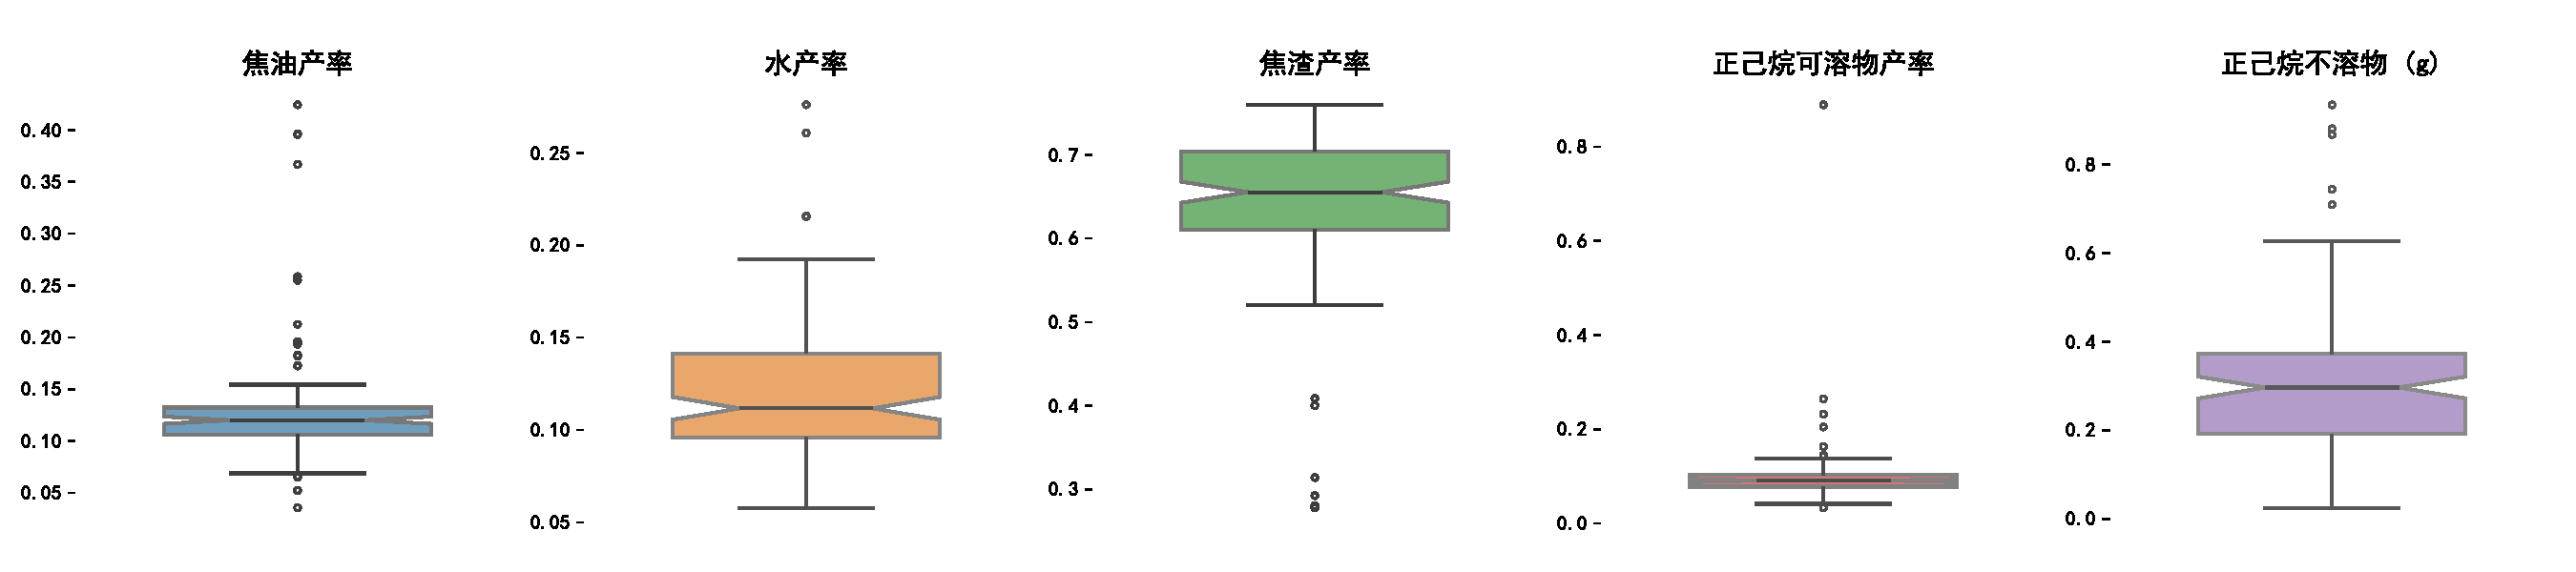
\includegraphics[width=0.99\linewidth]{pic/boxplot.pdf}
        \caption{关键变量箱线图}
        \label{fig:boxplot}
    \end{figure}
\end{frame}


\subsection{推理与总结}
\begin{frame}{推理与总结}
    \justifying
    通过数据预处理与探索性分析填补了数据缺失,且揭示了不同变量之间的内在联系。探索性数据分析的初步结论为后续的模型构建提供了重要的方向和依据:

    \begin{itemize}
        \item INS 含量与焦油产率显著相关,表明 INS 是影响焦油产率的关键因素之一。
        \item 生物质混合比例增加时,焦油和水产率上升,而焦渣产率下降。这一趋势反映了生物质高挥发分的特性。
        \item 数据中存在一定的线性与非线性关系,提示后续分析需综合考虑线性模型与非线性模型,以获得更精确的预测结果。
    \end{itemize}
    
    在接下来的研究中,我们将基于这些分析结果,进一步构建多元回归模型与集成模型,尝试捕捉各变量间更为复杂的交互作用,提升模型的预测精度与鲁棒性。
\end{frame}


% 模型建立与求解
\section{模型的建立与求解}

\subsection{问题一:INS对产率的影响分析}
\begin{frame}{问题一:INS对产率的影响分析}
    \justifying
    \begin{columns}
        \column{0.6\textwidth}
        \begin{block}{模型选择与理由}
            \begin{itemize}
                \item 选择\textbf{皮尔逊相关系数},度量INS与产物产率之间的线性相关性。
                \item 适用于连续变量,计算简便,结果易于解释。
            \end{itemize}
        \end{block}
        \begin{block}{皮尔逊相关系数公式}
            \[
            r = \frac{\sum_{i=1}^n (x_i - \bar{x})(y_i - \bar{y})}{\sqrt{\sum_{i=1}^n (x_i - \bar{x})^2} \sqrt{\sum_{i=1}^n (y_i - \bar{y})^2}}
            \]
        \end{block}
        \column{0.4\textwidth}
        \begin{block}{计算结果}
            \begin{table}[htbp]
                \centering
                \begin{tabular}{lcc}
                    \toprule
                    \textbf{变量关系} & \textbf{相关系数$r$} & \textbf{关系强度} \\
                    \midrule
                    INS与焦油产率 & 0.65 & 较强正相关 \\
                    INS与水产率 & 0.08 & 相关性弱 \\
                    INS与焦渣产率 & -0.41 & 中等负相关 \\
                    \bottomrule
                \end{tabular}
            \end{table}
        \end{block}
    \end{columns}
\end{frame}

\begin{frame}{问题一:结果分析与结论}
    \small
    \justifying
    \begin{columns}
        \column{0.5\textwidth}
        \begin{block}{结果解读}
            \begin{itemize}
                \item \textbf{INS与焦油产率}:INS含量增加有助于提高焦油产率。
                \item \textbf{INS与焦渣产率}:INS含量增加会降低焦渣产率。
                \item \textbf{INS与水产率}:相关性较弱,影响不明显。
            \end{itemize}
        \end{block}
        \begin{block}{结论}
            INS在热解过程中促进了焦油的生成,抑制了焦渣的形成,可能影响了热解反应的化学路径。
        \end{block}
        \column{0.5\textwidth}
        \begin{figure}[htbp]
            \centering
            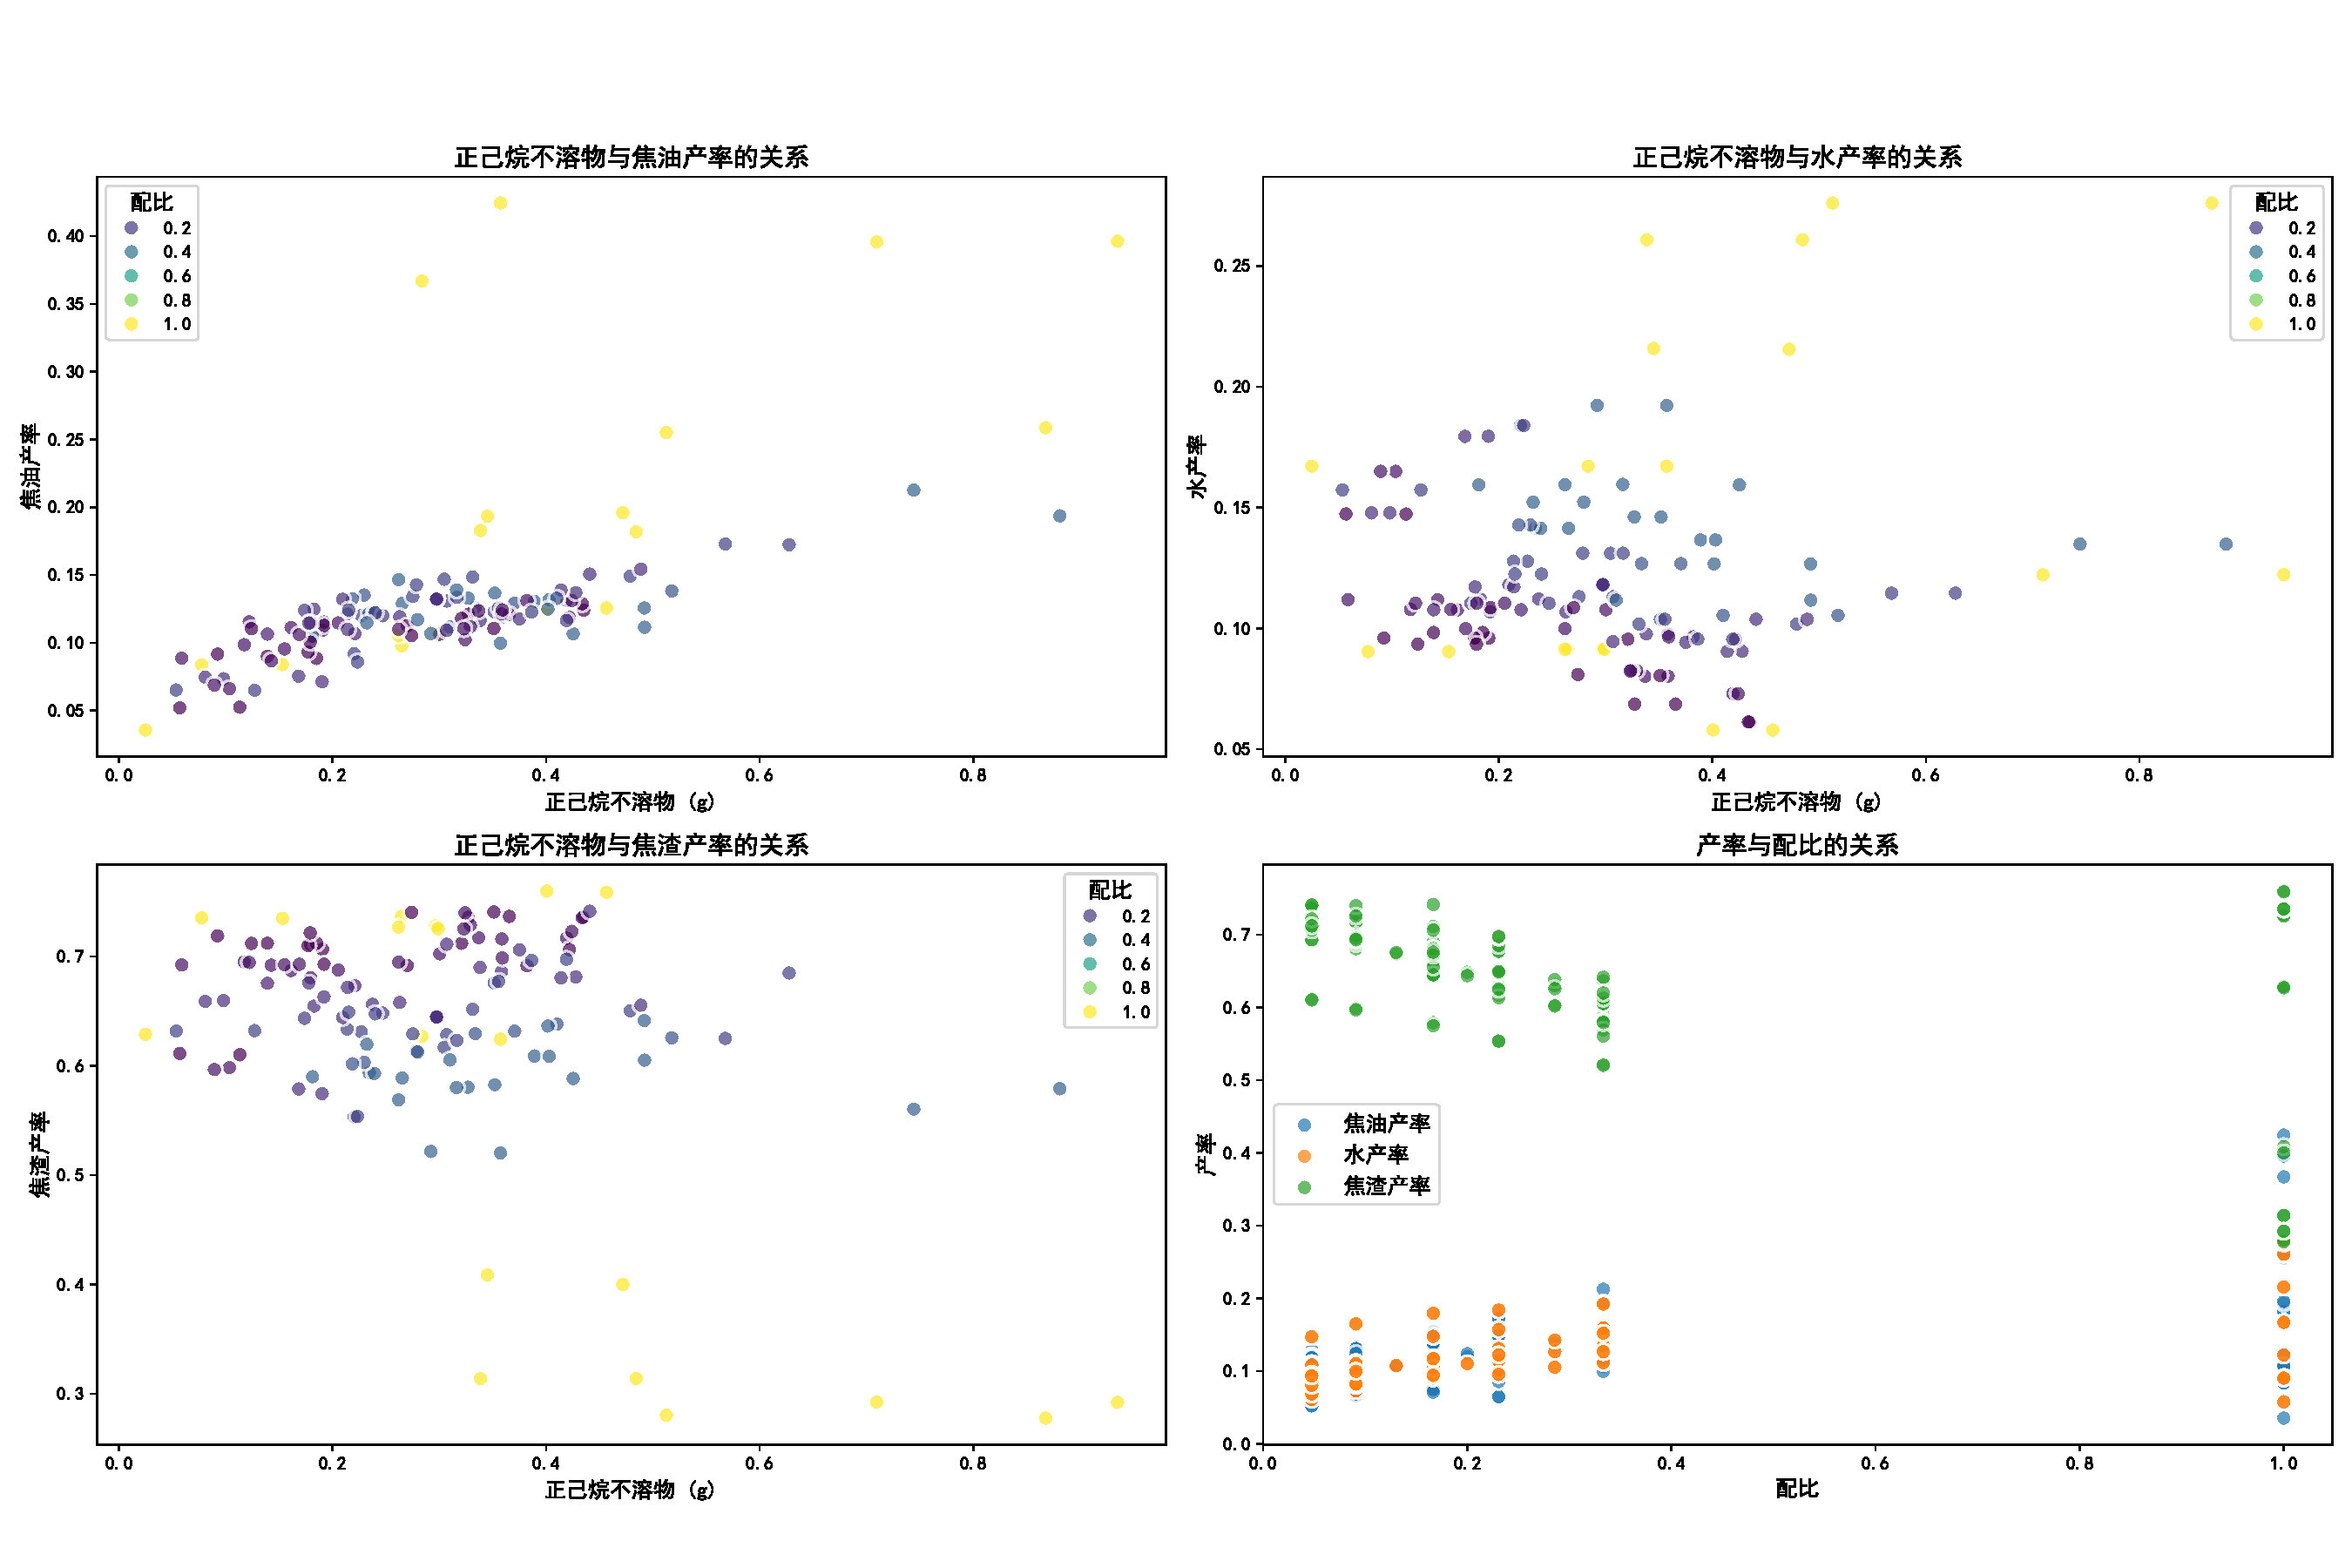
\includegraphics[width=\linewidth]{pic/scatterplot.pdf}
            \caption{INS与产物产率的关系}
            \label{fig:scatterplot}
        \end{figure}
        在散点图(图 \ref{fig:scatterplot})中呈现了生物质混合比例与焦油产率、焦渣产率、水产率的关系。随着生物质比例的增加,焦油和水的产率呈现上升趋势,而焦渣产率则下降。
    \end{columns}

\end{frame}

\subsection{问题二:INS与混合比例的交互效应}
\begin{frame}{问题二:INS与混合比例的交互效应}
    \justifying
    \begin{block}{模型选择与理由}
        \begin{itemize}
            \item 选择\textbf{LightGBM模型},处理高维特征和复杂非线性关系。
            \item 引入\textbf{交互特征}(INS $\times$ 配比),捕捉两者的协同作用。
        \end{itemize}
    \end{block}
    \begin{columns}
        \column{0.5\textwidth}
        \begin{block}{特征工程}
            \begin{itemize}
                \item \textbf{基础特征}:配比、样品质量、INS含量等。
                \item \textbf{交互特征}:INS $\times$ 配比。
            \end{itemize}
        \end{block}
        \column{0.5\textwidth}
        \begin{block}{模型训练与评估}
            \begin{itemize}
                \item 使用预处理后的数据,训练LightGBM模型。
                \item 通过交叉验证调整超参数,提升模型性能。
            \end{itemize}
        \end{block}
    \end{columns}
\end{frame}

\begin{frame}{问题二:特征重要性分析}
    \justifying
    \begin{columns}
        \column{0.6\textwidth}
        \begin{block}{结果解读}
            \begin{itemize}
                \item \textbf{交互特征}的重要性最高,表明INS与配比的协同效应显著影响焦油产率。
                \item \textbf{基础特征}的重要性次之,仍对产率有直接影响。
            \end{itemize}
        \end{block}
        \begin{block}{结论}
            优化热解工艺时,应同时考虑INS含量和混合比例,充分利用协同效应,提高产物产率。
        \end{block}
        \column{0.4\textwidth}
        \begin{figure}[htbp]
            \centering
            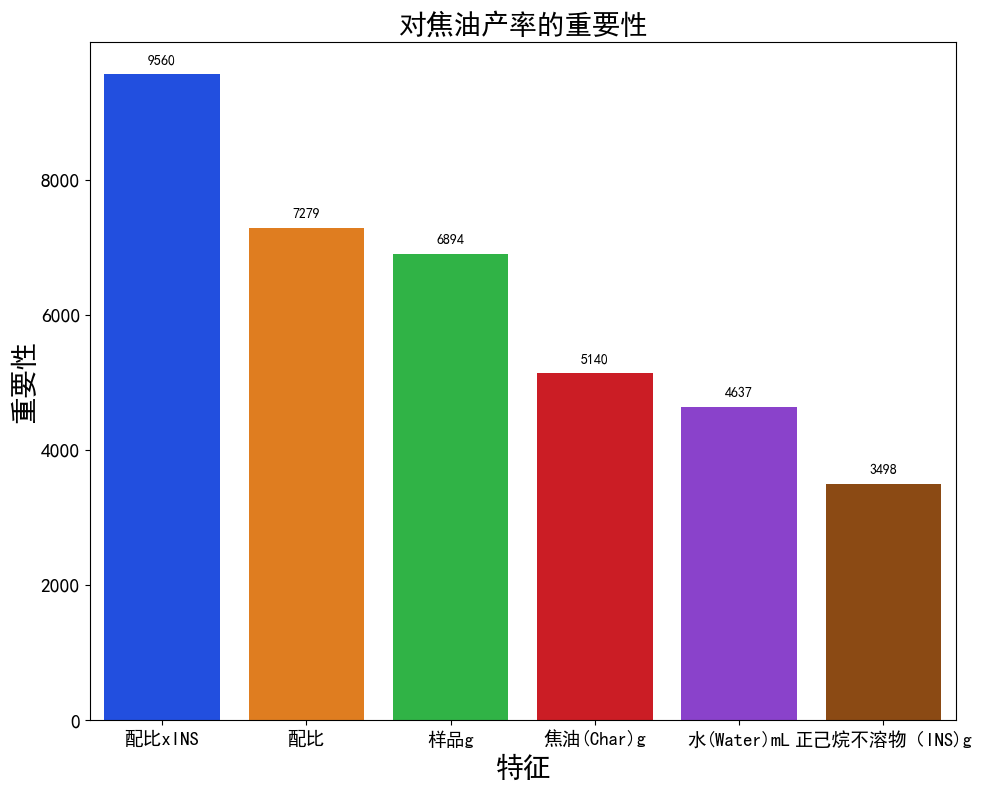
\includegraphics[width=\linewidth]{pic/焦油.png}
            \caption{焦油产率的特征重要性排名}
        \end{figure}
    \end{columns}
\end{frame}

% 问题三:最佳混合比例的确定
\subsection{问题三:最佳混合比例的确定}

\begin{frame}{问题三:最佳混合比例的确定}
    \begin{block}{问题分析}
        生物质-煤共热解过程涉及多个性能指标,核心要点为:
        \begin{itemize}
            \item 多目标性:需同时考虑产物利用率和能源转化效率
            \item 非线性关系:各因素间存在复杂的交互作用
            \item 数据限制:实验样本量有限,难以应用传统大数据方法
        \end{itemize}
    \end{block}
    \begin{block}{理论依据}
        \begin{enumerate}
            \item \textbf{熵权法}:基于信息论,能客观量化指标重要性
            \item \textbf{模糊综合评价}:处理多指标决策问题的有效工具,将多目标问题简化为单目标优化
            \item \textbf{多元多项式拟合}:捕捉变量间的非线性关系
            \item \textbf{粒子群优化(PSO)}:解决高维非凸优化问题
        \end{enumerate}
    \end{block}
\end{frame}

\begin{frame}{问题三:熵权法-模糊综合评价模型}
    \scriptsize
    \begin{block}{熵权法核心推导}
        给定 $m$ 个评价对象,$n$ 个指标,原始数据矩阵 $X = (x_{ij})_{m \times n}$:
        \[
            p_{ij} = \frac{x_{ij}}{\sum_{i=1}^m x_{ij}}, \quad
            E_j = -\frac{1}{\ln m}\sum_{i=1}^m p_{ij}\ln p_{ij}, \quad
            w_j = \frac{1-E_j}{\sum_{k=1}^n (1-E_k)}
        \]
    \end{block}
    \begin{block}{计算得到的评价指标权重}
        \centering
        \begin{tabular}{lcc}
            \toprule
            \textbf{指标} & \textbf{符号} & \textbf{权重 $w_j$} \\
            \midrule
            焦油产率 & $Y_\text{tar}$ & 0.3572 \\
            焦渣产率 & $Y_\text{char}$ & 0.2980 \\
            水产率 & $Y_\text{water}$ & 0.1981 \\
            正己烷可溶物产率 & $Y_\text{INS}$ & 0.1467 \\
            \bottomrule
        \end{tabular}
    \end{block}
\end{frame}

\begin{frame}{问题三:熵权法-模糊综合评价模型}
    \begin{block}{模糊综合评价实现目标融合}
        权重确定后,模糊综合评价将多个目标融合为单一目标。其步骤如下:
        \begin{itemize}
            \item 通过隶属函数将每个目标值标准化到区间 $[0,1]$。
            \item 对每个目标的隶属度进行加权求和:
            \[
                S = W \cdot R = \sum_{j=1}^m w_j \cdot r_j
            \]
            其中 $w_j$ 为权重,$r_j$ 为目标的隶属度,$S$ 为综合得分。
        \end{itemize}
        综合得分 $S$ 即为单一优化目标,从而实现将多目标问题简化为单目标优化。
    \end{block}
\end{frame}

\begin{frame}{问题三:熵权法-模糊综合评价模型}
    \begin{table}[htbp]
    \centering
    \caption{评价得分情况(部分展示)}
    \resizebox{\linewidth}{!}{
    \begin{tabular}{cccccc}
    \toprule
    \textbf{配比} & \textbf{样品g} & \textbf{焦油(Char)g} & \textbf{水(Water)mL} & \textbf{正己烷不溶物(INS)g} & \textbf{量化指标} \\
    \midrule
    1           & 10.5737      & 1.3179             & 0.58                & 0.400732     & 0.040207 \\
    1           & 10.2179      & 1.2832             & 0.59                & 0.4566       & 0.0326   \\
    1           & 10.3176      & 1.008171           & 0.943029            & 0.264736     & 0.003489 \\
    1           & 10.1371      & 1.075369           & 0.926531            & 0.296578     & 0.009528 \\
    1           & 9.299        & 0.9803             & 0.85                & 0.261862     & 0.007144 \\
    \bottomrule
    \end{tabular}}
    \label{table:score}
    \end{table}
\end{frame}

\begin{frame}{问题三:多元多项式拟合模型的构建与分析}
    \scriptsize
    \begin{block}{模型构建理论基础}
        基于 Taylor 展开理论,二阶多项式可以较好地逼近局部非线性关系:
        \[
            f(\mathbf{x}) \approx f(\mathbf{a}) + \nabla f(\mathbf{a})^T(\mathbf{x}-\mathbf{a}) + \frac{1}{2}(\mathbf{x}-\mathbf{a})^T H(\mathbf{a})(\mathbf{x}-\mathbf{a})
        \]
        其中,$H(\mathbf{a})$ 为 Hessian 矩阵。
    \end{block}
    \begin{block}{拟合模型及其分析}
        \scriptsize
        \[
            f(x_1,\ldots,x_5) = 0.119 + 0.176x_1 - 0.012x_2 - 0.120x_3 + 0.070x_4 - 0.071x_5 + \text{(交互项)}
        \]
        
        模型解释:
        \begin{itemize}
            \item $x_1$(配比)和 $x_4$(水)对目标函数有正面影响
            \item $x_2$(样品)、$x_3$(焦油)和 $x_5$(INS)呈负面影响
            \item R-squared 为 0.861528,表明模型解释了 86.15\% 的数据变异性
        \end{itemize}
    \end{block}
\end{frame}

\begin{frame}{问题三:粒子群优化算法的理论基础与应用}
    \scriptsize
    \begin{block}{PSO 算法的理论基础}
        基于群体智能理论,粒子的运动受三个因素影响:
        \begin{itemize}
            \item 惯性:保持当前运动趋势
            \item 认知:个体历史最优位置的吸引
            \item 社会:群体最优位置的吸引
        \end{itemize}
    \end{block}
    \begin{block}{算法核心公式及其解释}
        速度更新:
        \[
            v_{id}^{k+1} = \omega v_{id}^k + c_1r_1(p_{id}^k - x_{id}^k) + c_2r_2(p_{gd}^k - x_{id}^k)
        \]
        位置更新:
        \[
            x_{id}^{k+1} = x_{id}^k + v_{id}^{k+1}
        \]
        其中,$\omega$ 为惯性权重,$c_1$ 和 $c_2$ 分别为个体和群体学习因子。
    \end{block}
\end{frame}

\begin{frame}{问题三:结果分析与理论验证}\
    \small
    \begin{columns}[T]
        \column{0.52\textwidth}
        \begin{block}{优化结果及其物理意义}
            \begin{itemize}
                \item 最佳混合比例:\alert{28.44\%}
                \item 最大量化指标:0.3511
                \item 物理解释:在此比例下,生物质和煤的协同效应最强
            \end{itemize}
        \end{block}
        \begin{block}{与理论模型的一致性分析}
            \begin{itemize}
                \item 结果落在 30\% 临界值附近,符合文献\upcite{ref12}的预测
                \item 验证了低掺比下的正协同作用假说,提供了定量优化结果
            \end{itemize}
        \end{block}
        \column{0.48\textwidth}
        \begin{figure}
        \centering
        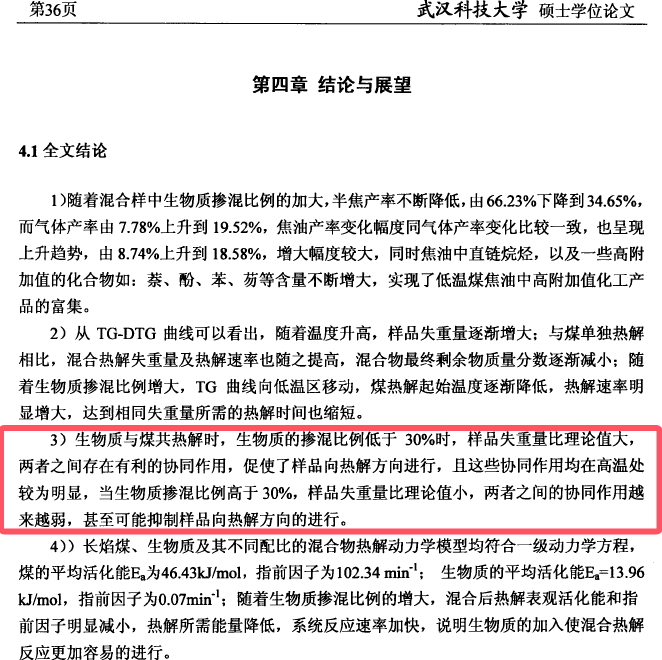
\includegraphics[width=\textwidth]{pic/文献结论.png}
        \caption{文献验证\upcite{ref12}}
        \end{figure}
    \end{columns}
\end{frame}

\subsection{问题四:差异显著的热解组合}
\begin{frame}{问题四:Wilcoxon符号秩检验差异性分析模型}
\small
\centering
\begin{tikzpicture}[
    node distance=1.8cm,
    auto,
    every node/.style={align=center},
    block_purple/.style={
        rectangle,
        draw,
        fill=purple!20,
        text width=4.2cm,
        rounded corners,
        minimum height=7em,
        font=\scriptsize
    },
    block_blue/.style={
        rectangle,
        draw,
        fill=blue!20,
        text width=4.2cm,
        rounded corners,
        minimum height=7em,
        font=\scriptsize
    },
    block_green/.style={
        rectangle,
        draw,
        fill=green!20,
        text width=4.2cm,
        rounded corners,
        minimum height=7em,
        font=\scriptsize
    },
    block_red/.style={
        rectangle,
        draw,
        fill=red!20,
        text width=4.2cm,
        rounded corners,
        minimum height=7em,
        font=\scriptsize
    },
    arrow/.style = {draw, -{Stealth[]}, thick}
]
    % 定义节点
    \node [block_purple] (theory) {
        \textbf{I. 理论基础与模型建立}\\[0.1cm]
        Wilcoxon符号秩检验原理\\
        模型假设:$H_0$ vs $H_1$\\
        统计量:$W = \min(W^+, W^-)$
    };
    \node [block_blue, right=1cm of theory] (data) {
        \textbf{II. 数据处理与准备}\\[0.1cm]
        数据重构:$\mathbf{A} = (a_{ij})$\\
        Lagrange插值:$L_n(x) = \sum\limits_{i=0}^n y_i \prod\limits_{j \ne i} \frac{x - x_j}{x_i - x_j}$\\
        差值计算:$D_{ij} = X_{ij} - Y_{ij}$
    };
    \node [block_green, below=1cm of theory] (analysis) {
        \textbf{III. 统计分析与检验}\\[0.1cm]
        Wilcoxon检验组间应用\\
        关键混合比例子组分析\\
        差异向量:$\mathbf{d}_j = (D_{1j}, \dots, D_{mj})^\top$
    };
    \node [block_red, right=1cm of analysis] (results) {
        \textbf{IV. 结果解释与推论}\\[0.1cm]
        6/40组存在显著差异\\
        差异主要在极端混合比例下
    };
    % 画箭头
    \draw [arrow] (theory) -- (data);
    \draw [arrow] (theory) -- (analysis);
    \draw [arrow] (data) -- (analysis);
    \draw [arrow] (analysis) -- (results);
\end{tikzpicture}

\vspace{0.2cm}
\justifying
\scriptsize
\textbf{方法选择理由:} 

采用\textbf{Wilcoxon符号秩检验},适用于\alert{小样本}和\alert{非正态分布}的数据,能够考虑差值的\alert{符号和大小},适合\alert{配对样本}的比较,对\alert{异常值不敏感},提高结果的稳健性。

\end{frame}

\begin{frame}{Wilcoxon符号秩检验运行结果}
    \justifying
    通过Wilcoxon符号秩检验,针对不同组别进行了组间和子组分析。以下展示了组间分析和各子组的检验结果。
    
    \vspace{0.3cm}
    
    \begin{figure}[htbp]
        \centering
        \begin{minipage}{0.4\linewidth}
            \centering
            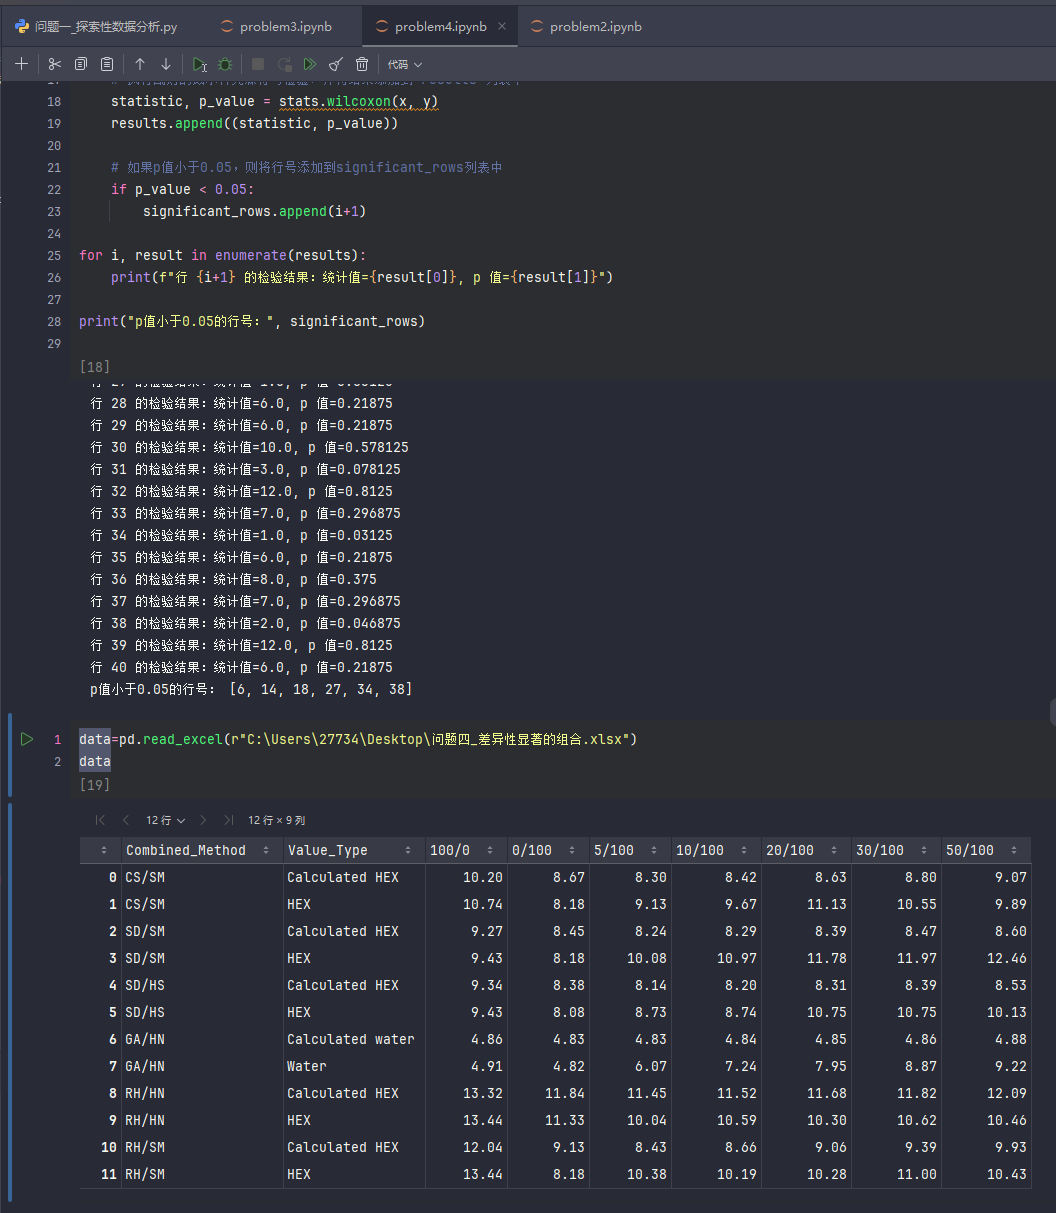
\includegraphics[width=\linewidth]{pic/path_to_image1.png} % 替换为实际路径
            \caption{组间分析}
        \end{minipage}
        \hspace{0.5cm}
        \begin{minipage}{0.4\linewidth}
            \centering
            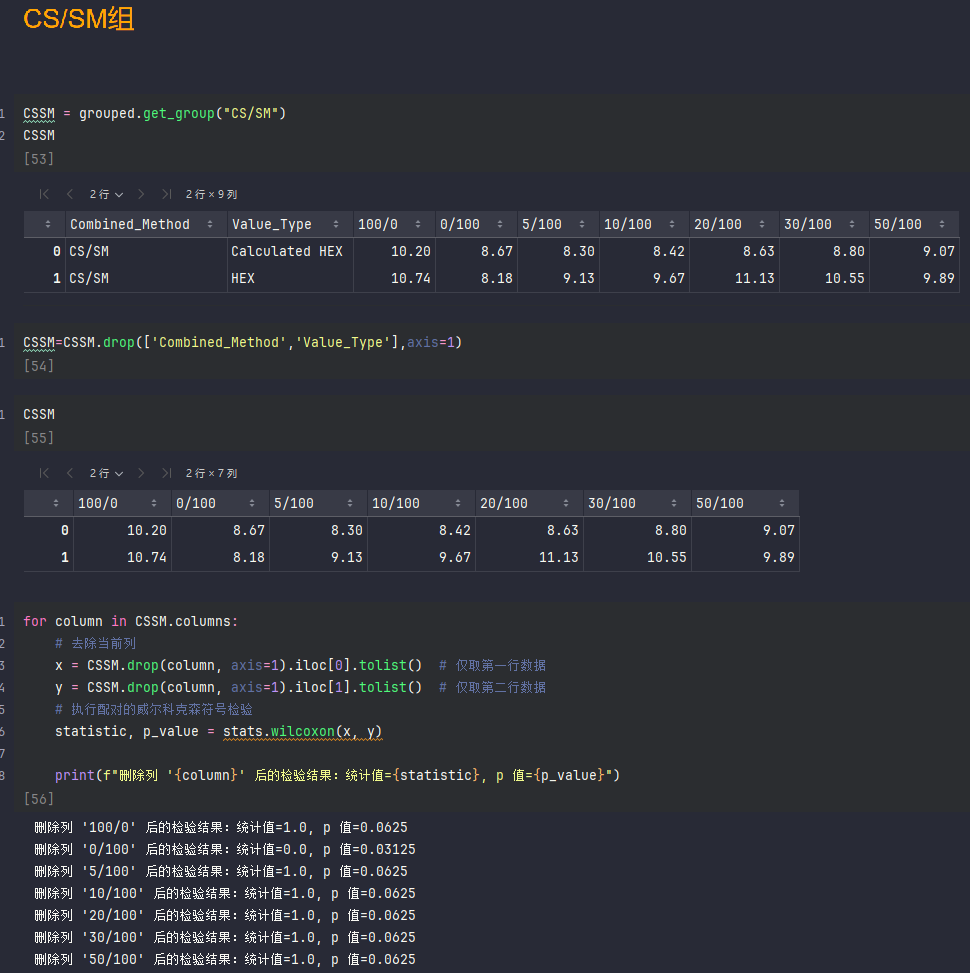
\includegraphics[width=\linewidth]{pic/path_to_image2.png} % 替换为实际路径
            \caption{CS/SM 组分析}
        \end{minipage}
    \end{figure}
\end{frame}

\begin{frame}{Wilcoxon符号秩检验运行结果}
    \justifying
        \vspace{0.3cm}
        \begin{figure}[htbp]
        \centering
        \begin{minipage}{0.4\linewidth}
            \centering
            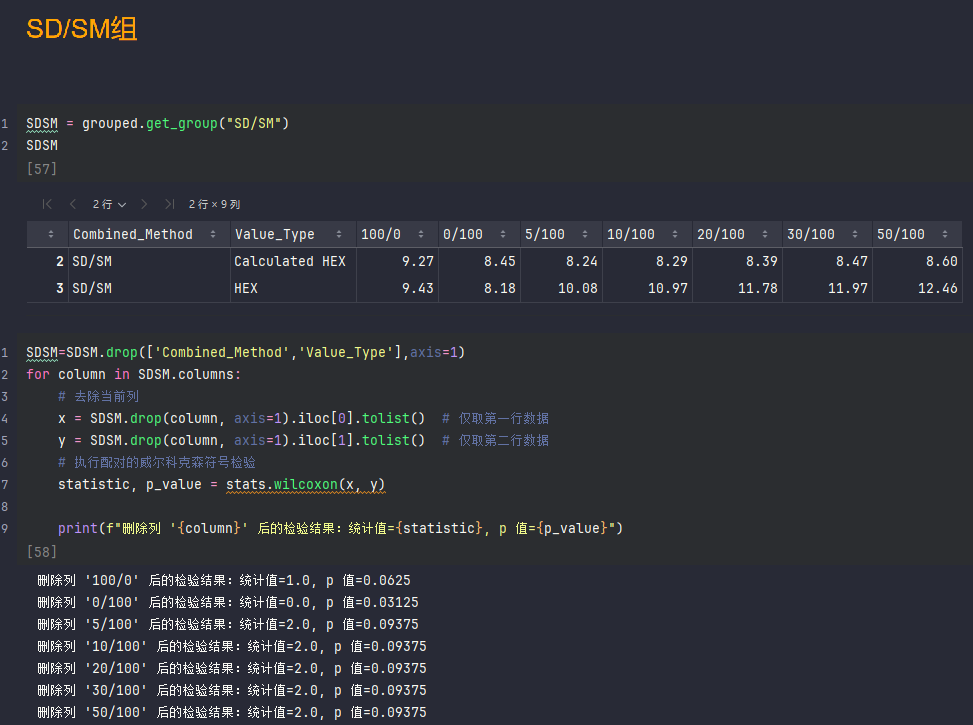
\includegraphics[width=\linewidth]{pic/path_to_image3.png} % 替换为实际路径
            \caption{SD/SM 组分析}
        \end{minipage}
        \hspace{0.5cm}
        \begin{minipage}{0.4\linewidth}
            \centering
            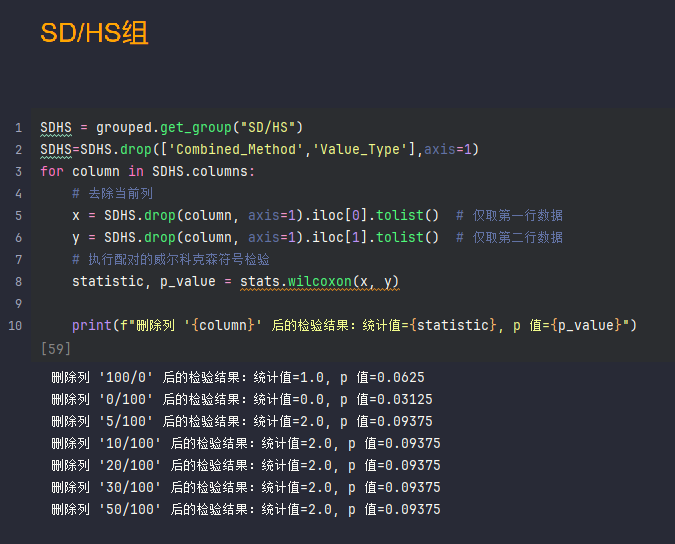
\includegraphics[width=\linewidth]{pic/path_to_image4.png} % 替换为实际路径
            \caption{SD/HS 组分析}
        \end{minipage}
    \end{figure}
\end{frame}

\begin{frame}{Wilcoxon符号秩检验运行结果}
    \justifying
        \begin{figure}[htbp]
        \centering
        \begin{minipage}{0.3\linewidth}
            \centering
            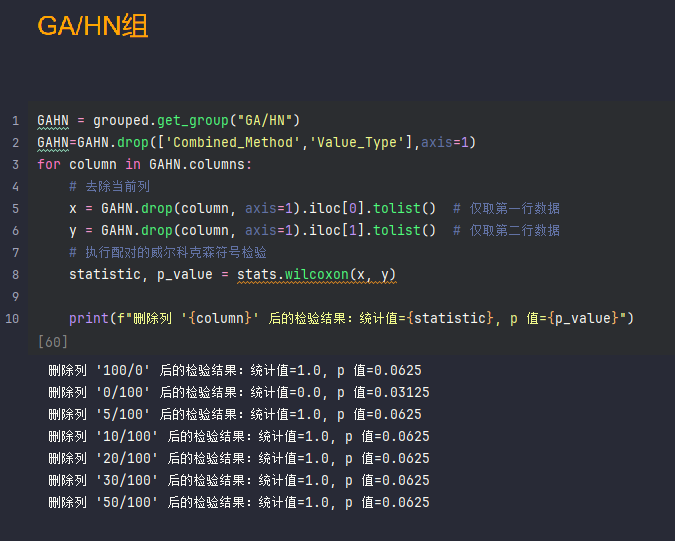
\includegraphics[width=\linewidth]{pic/path_to_image5.png} % 替换为实际路径
            \caption{GA/HN 组分析}
        \end{minipage}
        \begin{minipage}{0.3\linewidth}
            \centering
            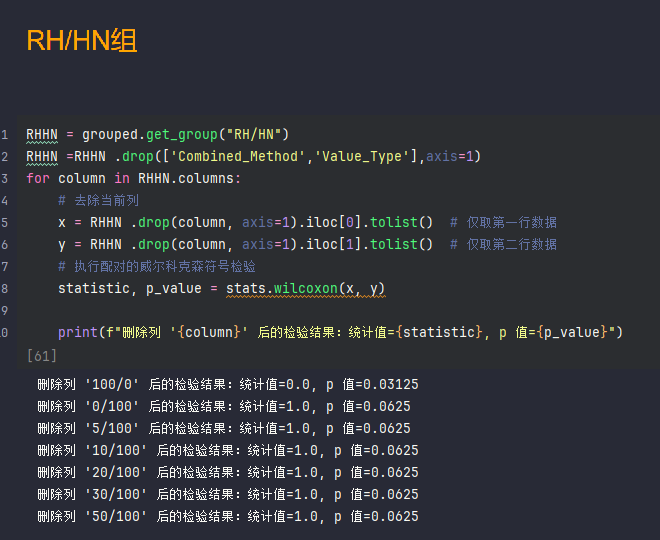
\includegraphics[width=\linewidth]{pic/path_to_image6.png} % 替换为实际路径
            \caption{RH/HN 组分析}
        \end{minipage}
        \begin{minipage}{0.3\linewidth}
            \centering
            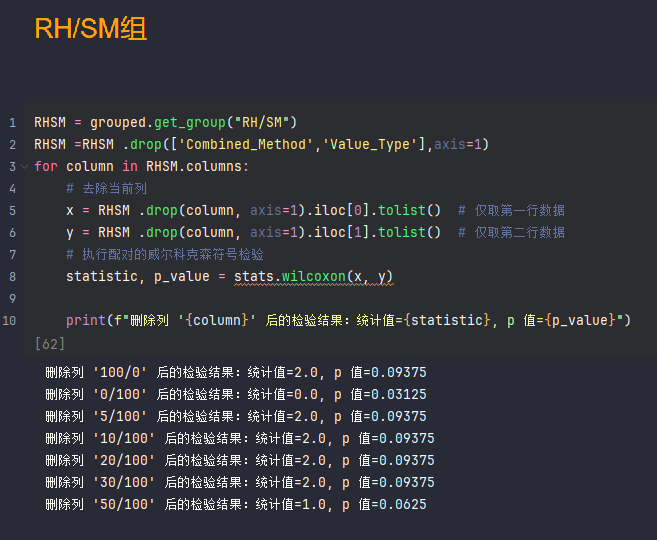
\includegraphics[width=\linewidth]{pic/path_to_image7.png} % 替换为实际路径
            \caption{RH/SM 组分析}
        \end{minipage}        
    \end{figure}
\end{frame}


\begin{frame}{问题四:差异显著的热解组合}
\centering
\begin{table}[htbp]
\scriptsize
\setlength{\tabcolsep}{4pt}
\begin{tabular}{cc|ccc}
\toprule
\multicolumn{2}{c|}{\textbf{差异显著的热解组合}} & \multicolumn{3}{c}{\textbf{共热解组合子组分析结果}} \\
\cmidrule(r){1-2} \cmidrule(l){3-5}
\textbf{组合} & \textbf{物质类型} & \textbf{组合} & \textbf{关键混合比例} & \textbf{剔除后 $p$ 值} \\
\midrule
CS/SM & HEX & CS/SM & 0/100 & 0.03125 \\
SD/SM & HEX & SD/SM & 0/100 & 0.03125 \\
SD/HS & HEX & SD/HS & 0/100 & 0.03125 \\
GA/HN & Water & GA/HN & 0/100 & 0.03125 \\
RH/HN & HEX & RH/HN & 100/0 & 0.03125 \\
RH/SM & HEX & RH/SM & 0/100 & 0.03125 \\
\bottomrule
\end{tabular}
\caption{差异显著的热解组合及子组分析结果}
\label{tab:significance}
\end{table}
\justifying
\small
\textbf{主要发现:}
在\alert{40组}实验中,有\alert{6组}存在显著差异,主要涉及\alert{HEX(正己烷)}产物。关键混合比例集中在\alert{纯煤(0/100)}和\alert{高比例生物质(100/0)},表明在\alert{极端混合比例}下,理论模型的预测准确性降低。非极性产物(HEX)的产率预测偏差较大,需进一步研究\alert{生物质与煤在极端比例下的相互作用机制},考虑改进理论模型,纳入更多\alert{影响因素}。
\end{frame}

\begin{frame}{不同生物质煤共热解与实验产物收率比较可视化}
    \begin{figure}[htbp]
    \centering
    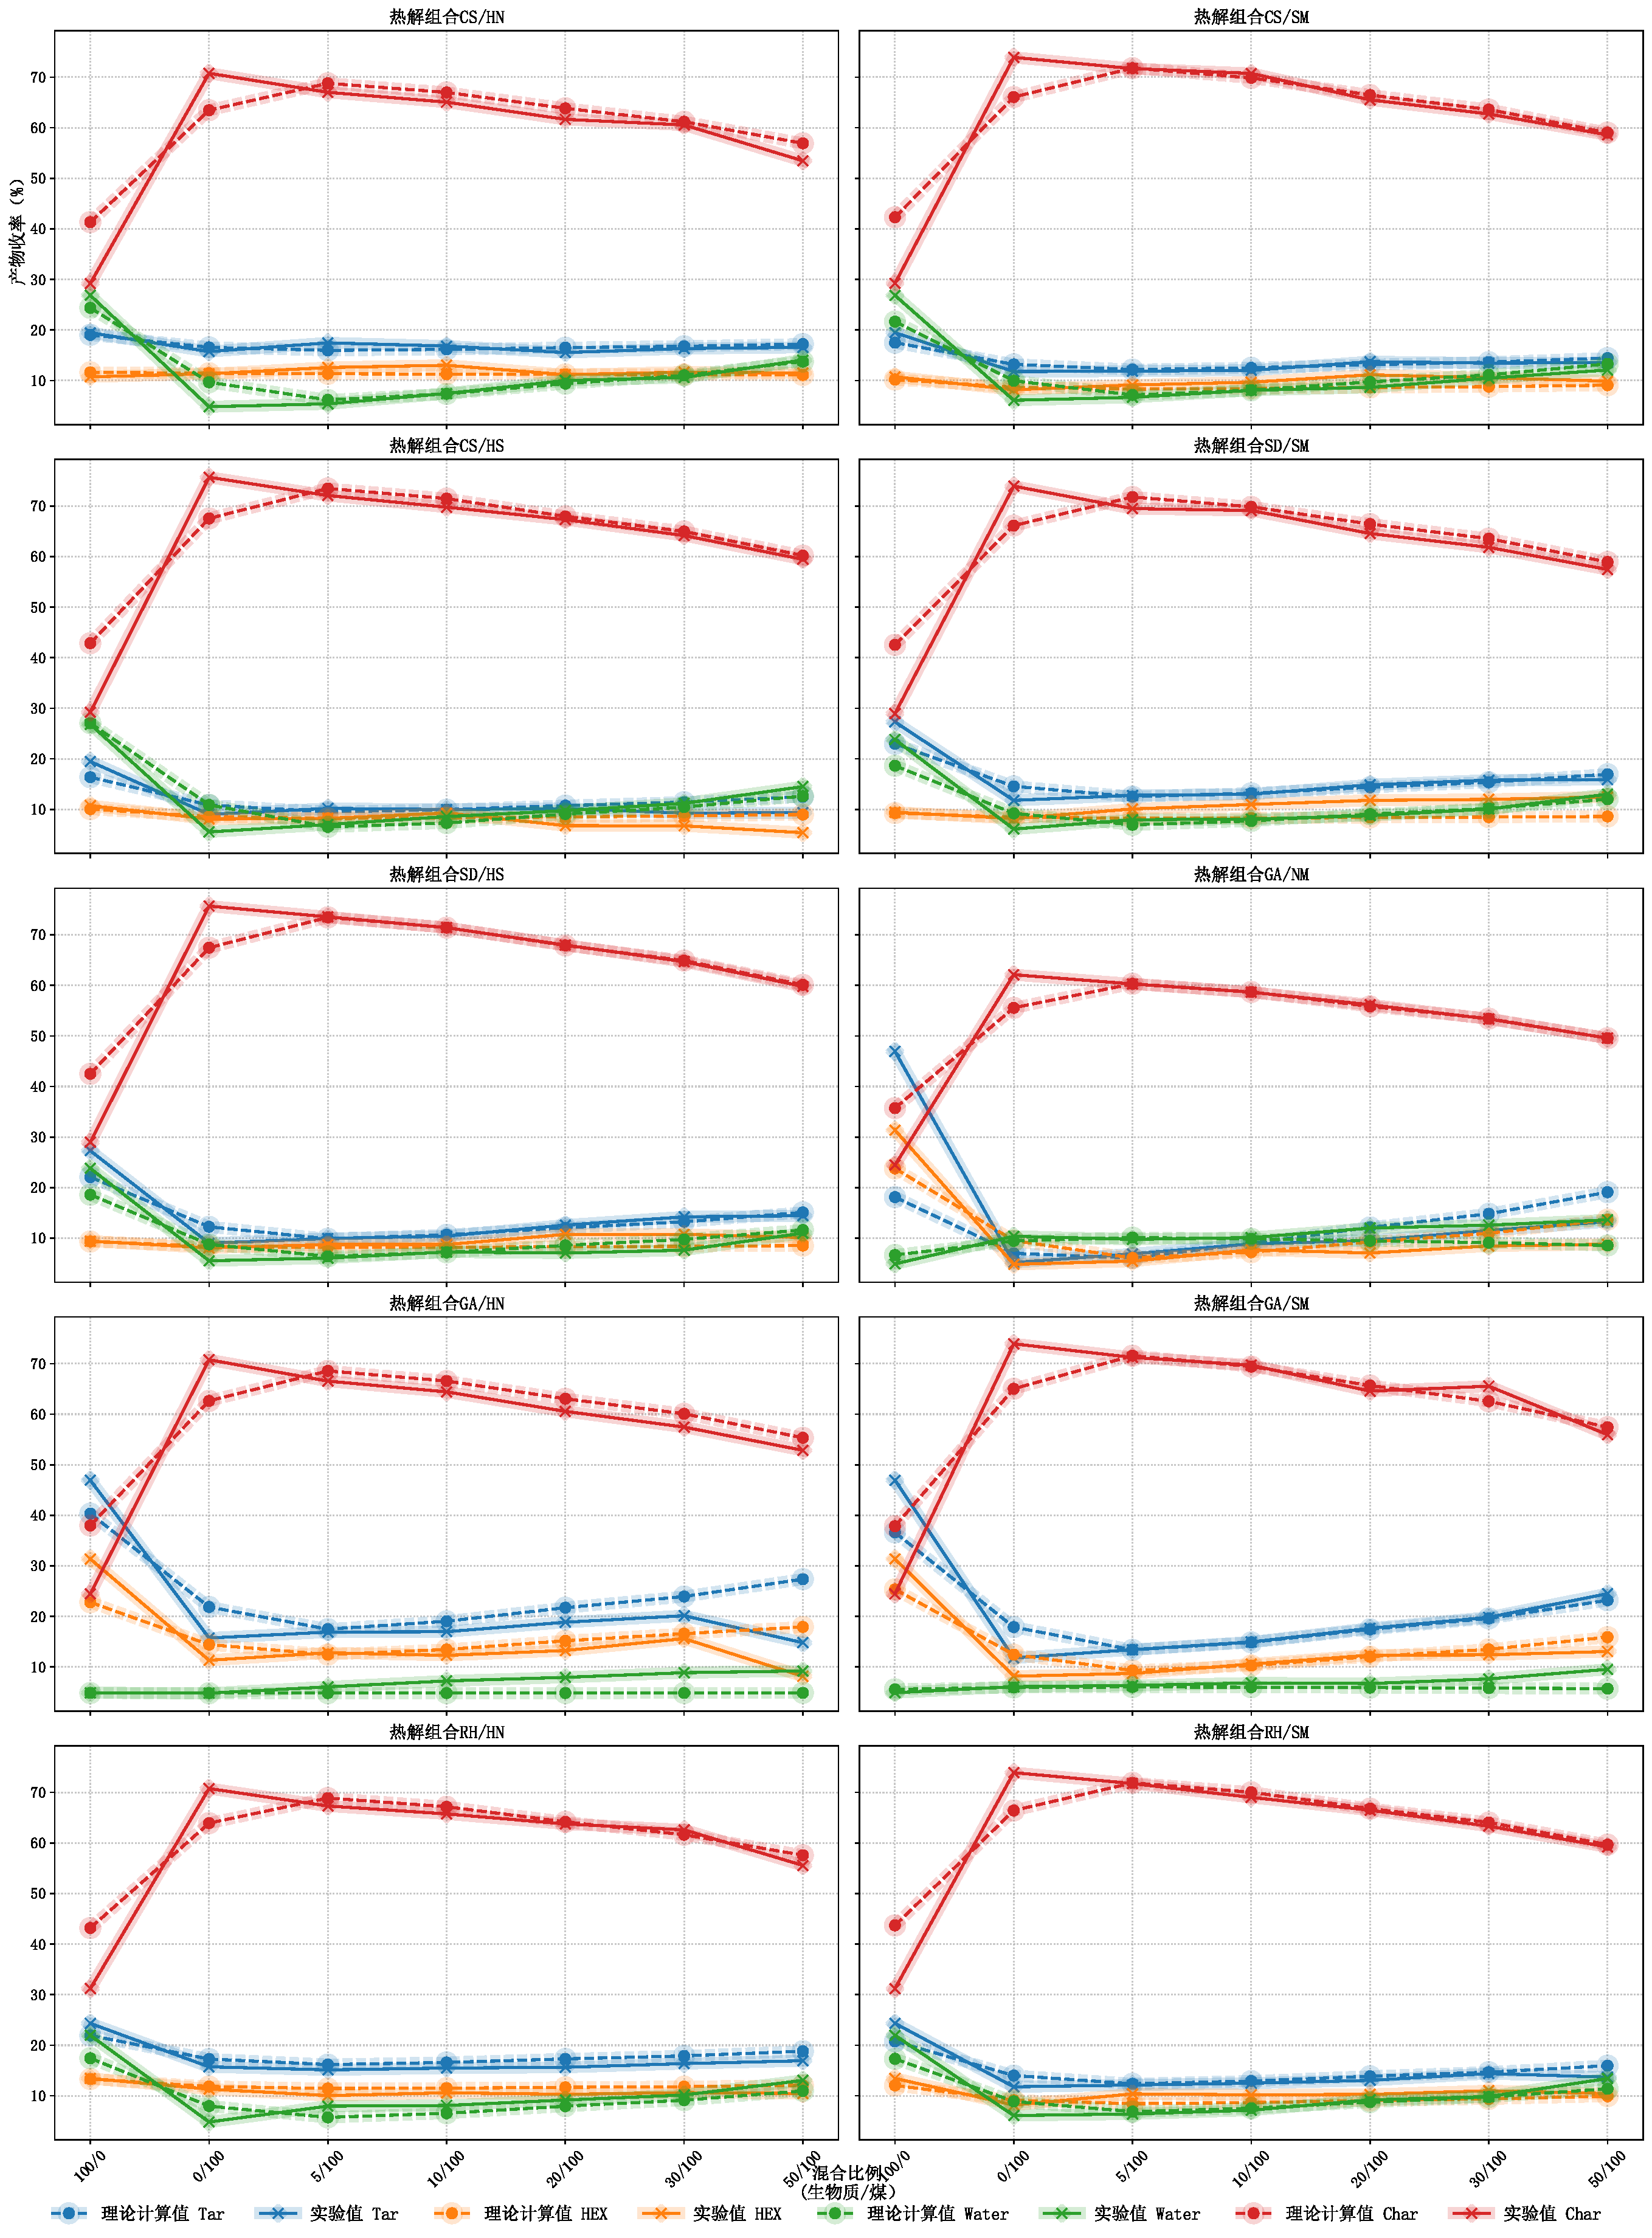
\includegraphics[width=0.5\linewidth]{pic/comparison_plots.pdf}
    \caption{不同生物质煤共热解与实验产物收率比较}
    \label{fig:comparison_plots}
    \end{figure}
\end{frame}

\subsection{问题五:热解产物产率预测模型}
\begin{frame}{问题五:热解产物产率预测模型 - 理论基础与方法选择}
    \scriptsize
    \begin{block}{问题分析}
        生物质-煤共热解过程是一个复杂的热化学转化过程,其产物产率预测涉及多个挑战:
        \begin{itemize}
            \item 多因素影响:配比、样品质量、焦油量、水量等因素共同作用。
            \item 非线性关系:因素间可能存在复杂的非线性交互作用。
            \item 数据特征:实验数据可能存在噪声和不确定性。
            \item 预测精度要求:需要在有限样本条件下实现高精度预测。
        \end{itemize}
        这些特点决定了我们需要选择能够适应复杂系统、捕捉非线性关系、并具有良好泛化能力的预测模型。
    \end{block}
    \begin{block}{理论依据}
        基于问题特性,我们选择了三种不同类型的模型:
        \begin{enumerate}
            \item \textbf{多元线性回归}:适合捕捉线性关系,提供基础因素分析。
            \item \textbf{随机森林回归}:非参数模型,适合处理非线性关系与复杂特征交互。
            \item \textbf{高斯过程回归}:非参数回归,在贝叶斯框架下优化选用,尝试量化不确定性并通过核函数捕捉复杂模式。
        \end{enumerate}
        这种多模型策略允许我们从不同角度分析问题,比较模型性能,并获得更全面的预测结果。
    \end{block}
\end{frame}

\begin{frame}{问题五:多元线性回归模型}
    \scriptsize
    \begin{block}{模型原理}
        多元线性回归模型假设因变量(热解产物产率)与自变量(影响因素)之间存在线性关系:
        \[y = \beta_0 + \beta_1 x_1 + \beta_2 x_2 + \cdots + \beta_p x_p + \varepsilon\]
        其中,$y$ 为焦油产率,$x_i$ 为影响因素,$\beta_i$ 为回归系数,$\varepsilon$ 为随机误差项。
        
        模型估计采用最小二乘法,最小化残差平方和:
        \[\min_{\beta} \sum_{i=1}^n (y_i - (\beta_0 + \beta_1 x_{i1} + \cdots + \beta_p x_{ip}))^2\]
        
        通过求解正规方程 $(X^T X)\beta = X^T y$,我们可以得到参数估计 $\hat{\beta} = (X^T X)^{-1} X^T y$。
    \end{block}
\end{frame}
\begin{frame}{问题五:多元线性回归模型}
    \begin{block}{参数估计结果与解释}
        拟合得到的模型为:
        \[\hat{y} = 0.0000 - 0.3108x_1 - 0.0431x_2 + 0.0194x_3 + 0.7672x_4\]
        其中,$x_1$: 配比,$x_2$: 样品质量,$x_3$: 焦油量,$x_4$: 水量。
        
        解释:
        \begin{itemize}
            \item 配比($x_1$)和样品质量($x_2$)对产率有负面影响,可能是由于高配比和大样品量导致热解不充分。
            \item 焦油量($x_3$)和水量($x_4$)对产率有正面影响,特别是水量的影响最为显著(系数最大)。
        \end{itemize}
    \end{block}
\end{frame}

\begin{frame}{问题五:多元线性回归模型结果可视化}
    \scriptsize
    \begin{figure}
        \centering
        \begin{minipage}[t]{0.45\linewidth}
            \centering
            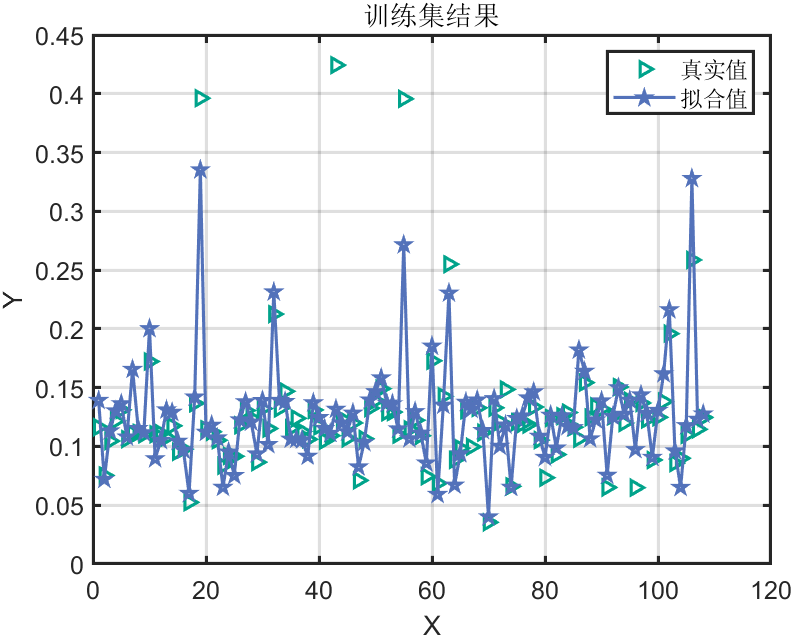
\includegraphics[width=\linewidth]{pic/线性回归训练集.png}
            \caption{训练集拟合结果}
            \label{fig:train_fit}
        \end{minipage}%
        \hfill
        \begin{minipage}[t]{0.45\linewidth}
            \centering
            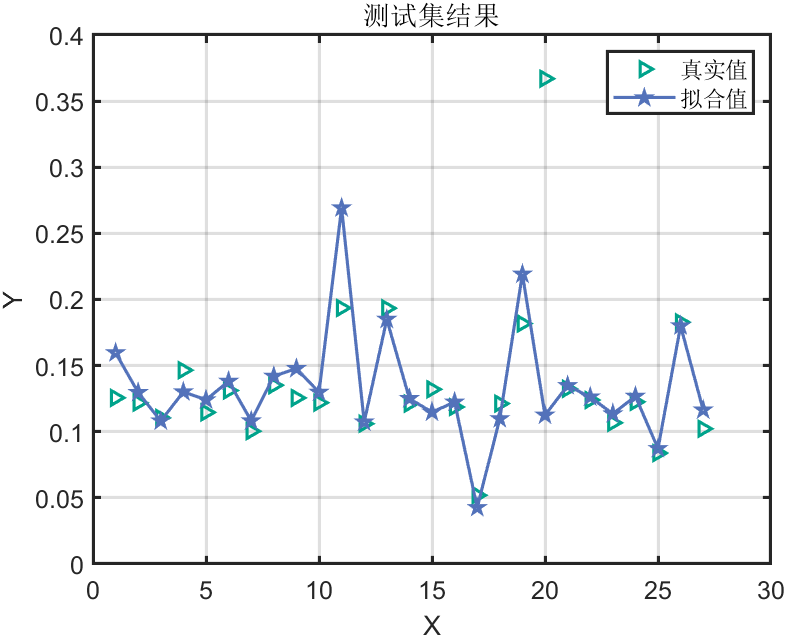
\includegraphics[width=\linewidth]{pic/线性回归测试集.png}
            \caption{测试集预测结果}
            \label{fig:test_prediction}
        \end{minipage}
    \end{figure}

    \vspace{0.2cm}
    
    从图中可以看出,模型在训练集上具有较好的拟合度,但在测试集上仍然存在一定的偏差,表明线性模型可能无法完全捕捉系统中的非线性特征。
\end{frame}

\begin{frame}{问题五:随机森林回归模型}
    \scriptsize
    \begin{block}{模型原理}
        随机森林是一种集成学习方法,通过构建多个决策树并结合它们的预测来进行回归:
        \begin{itemize}
            \item 基于 Bootstrap 采样构建多个决策树,每棵树使用随机选择的特征子集。
            \item 决策树生长过程中,节点分裂基于最小化不纯度(如 Gini 指数或均方误差)。
            \item 最终预测通过平均所有决策树的预测结果得到。
        \end{itemize}
    \end{block}
    \begin{block}{模型优势与局限性}
        \textbf{优势}:
        \begin{itemize}
            \item 随机森林能够有效处理非线性关系和特征交互。
            \item 不受多重共线性影响,适用于高维数据。
            \item 可以评估特征重要性,具有良好的解释性。
        \end{itemize}
        \textbf{局限性}:
        \begin{itemize}
            \item 模型复杂度高,训练和预测时间可能较长。
            \item 难以捕捉超出训练数据范围的模式(外推能力有限)。
            \item 可能出现过拟合,尤其是当树的数量不足或深度过大时。
        \end{itemize}
    \end{block}
\end{frame}

\begin{frame}{问题五:随机森林模型结果可视化}
    \scriptsize
    \begin{figure}
        \centering
        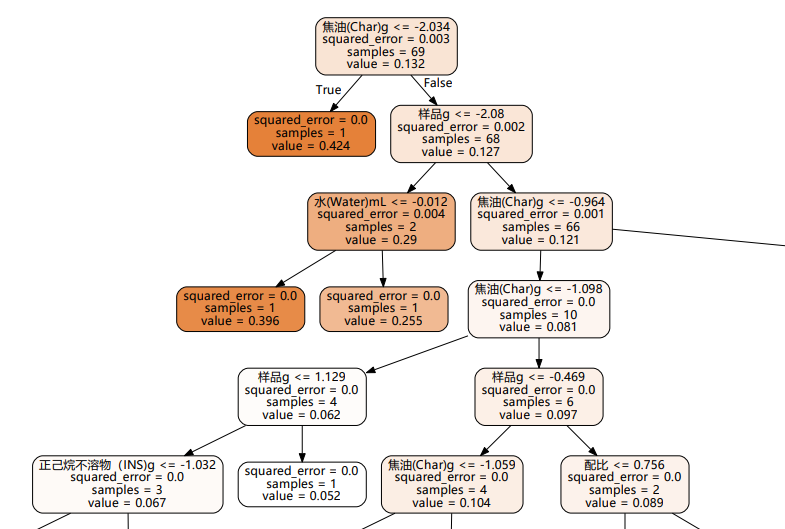
\includegraphics[width=0.8\linewidth]{pic/决策树.png}
        \caption{随机森林中的一棵决策树部分可视化}
        \label{fig:treevis}
    \end{figure}
\end{frame}

\begin{frame}{问题五:贝叶斯优化-高斯过程回归模型}
    \scriptsize
    \begin{block}{模型原理}
        高斯过程回归(GPR)是一种基于贝叶斯框架的非参数回归方法:
        \[f(x) \sim \mathcal{GP}(m(x), k(x,x'))\]
        其中,$m(x)$ 是均值函数,$k(x,x')$ 是协方差函数(即核函数),通常采用RBF核:
        \[k(x,x') = \sigma_f^2 \exp(-\frac{1}{2l^2}||x-x'||^2)\]
        该模型能够量化预测的不确定性,并通过核函数捕捉复杂的非线性关系。
    \end{block}
    \begin{block}{贝叶斯优化与超参数选择}
        \begin{itemize}
            \item 贝叶斯优化可以帮助我们自动调整GPR的超参数(如$\sigma_f^2$、$l$、$\sigma_n^2$),以提高模型性能。
            \item 通过最大化边际似然(或最小化负对数边际似然)来选择最优的超参数组合。
        \end{itemize}
    \end{block}
\end{frame}

\begin{frame}{问题五:贝叶斯优化-高斯过程回归模型结果可视化}
    \scriptsize
    \begin{figure}
        \centering
        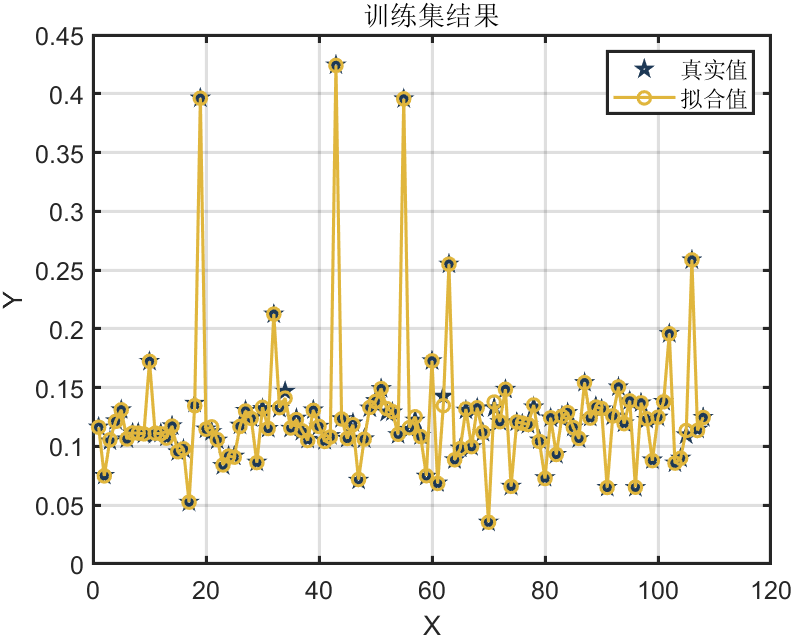
\includegraphics[width=0.32\linewidth]{pic/高斯回归+贝叶斯优化-训练集.png}
        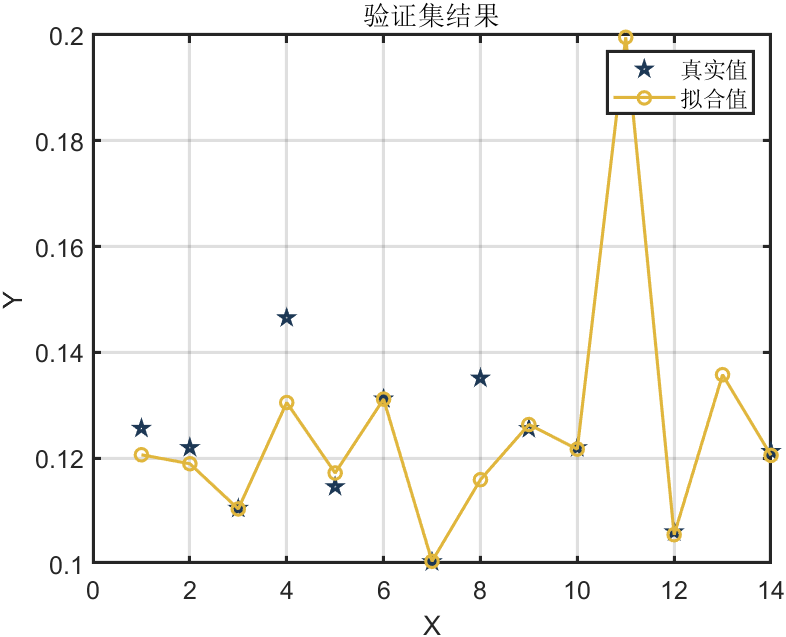
\includegraphics[width=0.32\linewidth]{pic/高斯回归+贝叶斯优化-验证集.png}
        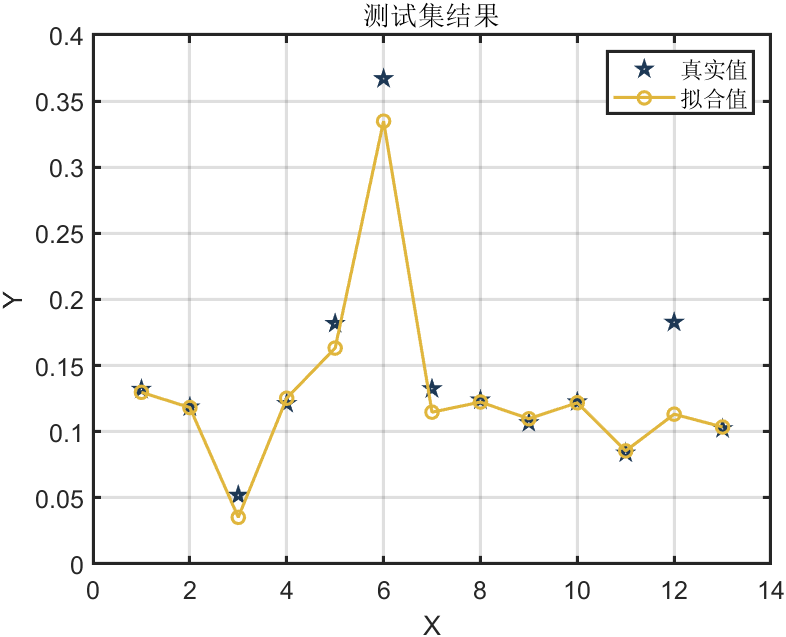
\includegraphics[width=0.32\linewidth]{pic/高斯回归+贝叶斯优化-测试集.png}
        \caption{高斯回归-贝叶斯优化模型结果}
        \label{fig:gaussian_bayesian_results}
    \end{figure}
\end{frame}

\begin{frame}{模型性能比较与结果分析}

    \begin{block}{评估指标对比}
        \centering
        \begin{tabular}{lccc}
            \toprule
            \textbf{模型} & \textbf{MAE} & \textbf{MSE} & \textbf{RMSE} \\
            \midrule
            线性回归 & 0.0215 & 0.0028 & 0.0527 \\
            随机森林 & 0.0201 & 0.0031 & 0.0561 \\
            高斯过程 & \textbf{0.0130} & \textbf{0.0005} & \textbf{0.0229} \\
            \bottomrule
        \end{tabular}
    \end{block}

    \vspace{0.1cm} % 添加适当的间隔以使版面更加美观

    \begin{block}{结果分析}
        \begin{itemize}
            \item 高斯过程回归在所有指标上都优于其他两种方法,特别是在 MAE 和 RMSE 方面有显著改善。
            \item 随机森林在捕捉非线性特征方面表现不错,但在 MSE 和 RMSE 上的表现稍逊。
            \item 线性回归由于其线性假设,在捕捉复杂特征方面表现不佳。
        \end{itemize}
    \end{block}
\end{frame}

\subsection{研究展望}
\begin{frame}{研究展望}
    \justifying
    \begin{columns}
        \column{0.5\textwidth}
        \begin{block}{未来工作方向}
            \begin{itemize}
                \item \textbf{模型改进}:考虑更多影响因素,设计多优化目标模型。
            \end{itemize}
        \end{block}
        \column{0.5\textwidth}
        \begin{block}{实际应用}
            \begin{itemize}
                \item \textbf{工业实践}:将模型应用于工业生产,验证其可行性和有效性。
            \end{itemize}
        \end{block}
    \end{columns}
\end{frame}

% 参考文献
\section*{参考文献}
\begin{frame}[allowframebreaks]{参考文献}
    \tiny
    \begin{thebibliography}{9}  
        \bibitem{ref13} 何玉远,常春,方书起,陈俊英,李洪亮,马晓建. 煤与生物质共热解工艺的研究进展[J]. 可再生能源, 2018, 36(2):159-166. DOI:10.3969/j.issn.1671-5292.2018.02.001    
        \bibitem{ref12} 潘叶. 生物质与低阶煤低温共热解转化研究[D]. 武汉科技大学, 2013.
        \bibitem{ref1} 赵源上, 林伟芳. 基于皮尔逊相关系数融合密度峰值和熵权法典型场景研究[J]. 中国电力, 2023, 56(05):193-202.
        \bibitem{ref6} Dehua Wang, Yang Zhang, and Yi Zhao. LightGBM: An Effective miRNA Classification Method in Breast Cancer Patients. In Proceedings of the 2017 International Conference on Computational Biology and Bioinformatics (ICCBB '17). Association for Computing Machinery, New York, NY, USA, 7–11.
        \bibitem{ref7} Al-Kasassbeh M, Abbadi M A, Al-Bustanji A M. LightGBM algorithm for malware detection[C]//Intelligent Computing: Proceedings of the 2020 Computing Conference, Volume 3. Springer International Publishing, 2020: 391-403.
        \bibitem{ref2} 符学葳. 基于层次分析法的模糊综合评价研究和应用[D]. 哈尔滨工业大学, 2011.
        \bibitem{ref3} 周文华, 王如松. 基于熵权的北京城市生态系统健康模糊综合评价[J]. 生态学报, 2005, (12):3244-3251.
        \bibitem{ref4} 杨辉, 李昕涛, 王茹愿, 等. 基于粒子群算法的开关磁阻电机控制系统研究[J]. 微特电机, 2024, 52(04):65-71. DOI:10.20026/j.cnki.ssemj.2024.0059.
        \bibitem{ref5} 张宏韬, 唐芳, 吴坤, 等. 基于粒子群优化BP神经网络的激光扫描投影系统畸变预测方法[J/OL]. 光子学报, 2024. http://kns.cnki.net/kcms/detail/61.1235.O4.20240509.0902.004.html.
        \bibitem{ref8} 游晋峰, 安莹. 基于多元多项式回归的空气质量数据校准模型[J]. 山东商业职业技术学院学报, 2020, 20(06):91-99. DOI:10.13396/j.cnki.jsict.2020.06.020.
        \bibitem{ref9} 王峰, 郭金禄, 郑煜. 基于多元多项式回归的大兴安岭过火面积与气象因子的模型[J]. 森林工程, 2014, 30(03):56-58. DOI:10.16270/j.cnki.slgc.2014.03.030.
        \bibitem{ref10} Segal M R. Machine learning benchmarks and random forest regression[J]. 2004.
        \bibitem{ref11} 李彩琳, 宋彦涛, 张靖, 等. 基于随机森林算法的羌塘草原NDVI时空格局及其预测模型[J/OL]. 生态学杂志, 2024. http://kns.cnki.net/kcms/detail/21.1148.Q.20240313.1624.010.html.
        \bibitem{li2014gaussian} 李振刚. 基于高斯过程回归的网络流量预测模型[J]. 计算机应用, 2014, 34(5):1251-1254. DOI: http://www.joca.cn/CN/10.11772/j.issn.1001-9081.2014.05.1251.
    \end{thebibliography}
\end{frame}

% 致谢与答辩
\section*{致谢与答辩}
\begin{frame}{致谢与答辩}
    \justifying
    \begin{itemize}
        \item 首先,感谢指导老师对团队参加"数维杯"的支持。
        \item 特别感谢"数维杯"组委会提供的宝贵机会和展示平台。
        \item 最后,感谢各位评委老师的聆听与指导。恭请评委老师提出问题。
    \end{itemize}
    \vspace{1cm}
    \begin{center}
         {\Huge\textbf{感谢您的聆听!}}
    \end{center}
\end{frame}

\end{document}
